\resizebox{\columnwidth}{!}{
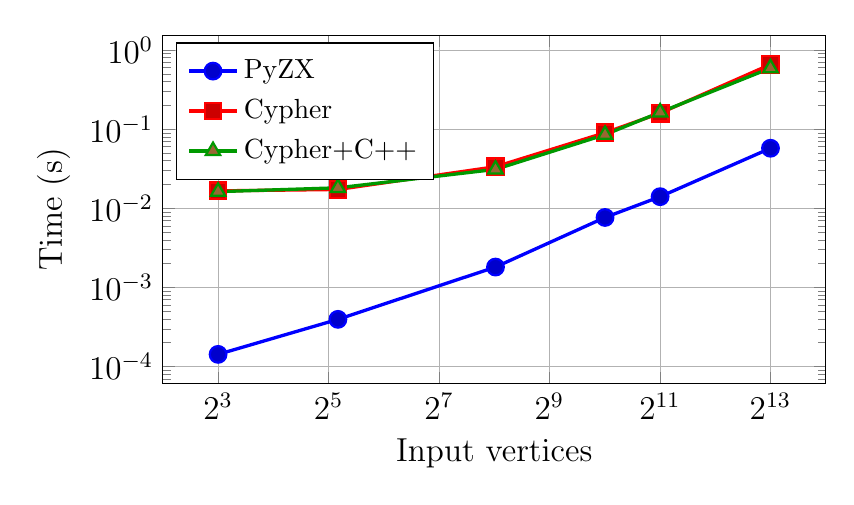
\begin{tikzpicture}
  \begin{axis}[
    width=10cm, height=6cm,
    xlabel={Input vertices}, ylabel={Time (s)},
    xmode=log, ymode=log, log basis x=2,
    grid=major,
    grid style={line width=.1pt, draw=gray!30},
    major grid style={line width=.2pt, draw=gray!60},
    label style={font=\large}, tick label style={font=\large},
    legend style={at={(0.02,0.98)}, anchor=north west,
      font=\normalsize, inner sep=4pt, row sep=2pt, cells={anchor=west}},
    legend image post style={mark size=3pt},
    every axis plot/.append style={line width=1.2pt, mark size=3pt,
      mark options={line width=0.8pt}},
    unbounded coords=jump,
  ]
    \addplot+[mark=*, color=blue, solid,error bars/.cd,y dir=both,y explicit] coordinates {
      (8,0.000142700002)
      (36,0.000395300001)
      (260,0.0018113)
      (1028,0.0076674)
      (2052,0.0140282)
      (8196,0.0574602)
    };
    \addlegendentry{PyZX}

    \addplot+[mark=square*, color=red, solid,error bars/.cd,y dir=both,y explicit] coordinates {
      (8,0.0166109)
      (36,0.0173102)
      (260,0.0335254)
      (1028,0.0901972)
      (2052,0.159417)
      (8196,0.6580402)
    };
    \addlegendentry{Cypher}

    \addplot+[mark=triangle*, color=green!60!black, solid,error bars/.cd,y dir=both,y explicit] coordinates {
      (8,0.0162468)
      (36,0.0181587)
      (260,0.0310405)
      (1028,0.0852487)
      (2052,0.1635874)
      (8196,0.591376)
    };
    \addlegendentry{Cypher+C++}

  \end{axis}
\end{tikzpicture}
}
